We now consider the case of random interactions.
Speficially, we assume that interaction coefficients $A_{ij}$ are drawn independently from a distribution with mean $\mu$ and standard deviation $\sigma$;
We assume the diagonal elements $A_{ii}$ have a mean value $\mu_s$ (possibly different from $\mu$) but the same standard deviation $\sigma$. 
 
We compute the Jacobian matrix at equilibrium
\begin{align}
    J_{ij}^* & = A_{ij}g(x_i^*)h'(x_j^*) \qquad \qquad \textrm{for} \ i\neq j \label{eq: jac off-diag}\\
    J_{ii}^* & = f'(x_i^*) - g'(x_i^*)f(x_i^*)/g(x_i^*) + A_{ii}g(x_i^*)h'(x_j^*) \ , \label{eq: jac diag}
\end{align}
where we used $\sum_{j}A_{ij}h(x_j^*)=-f(x_i^*)/g(x_i^*)$.
In order to investigate the spectral properties of $J^*$, 
we follow Stone~\cite{Stone2018} in using a recent generalization of the circular law in random matrix theory~\cite{Ahmadian2015}.

In Ref.~\cite{Ahmadian2015}, Ahmadian \emph{et al.} consider matrices of the form $M + LSR$, where $M$,  
$L$ and $R$ are deterministic matrices, and $S$ is a random matrix with i.i.d. coefficients, zero mean and variance $\sigma^2$.
They show that eigenvalues of large matrices of this form are contained in the complex domain $\mathcal{D} = \{\zeta \in \mathbb{C},\, \textrm{Tr}[(\Psi(\zeta) \Psi(\zeta)^\dagger)^{-1}]\geq \sigma^{-2}\}$, where $\Psi(\zeta) = L^{-1}(M-\zeta I)R^{-1}$. If $L$, $R$ and $M$ are all diagonal $N\times N$ matrices, the equation of $\mathcal{D}$ simplifies to 
\begin{equation}
    \sum_{i=1}^N\Big\vert\frac{M_{ii} - \zeta}{L_{ii}R_{ii}}\Big\vert^{-2}\geq \sigma^{-2}.
\label{eq: domain}
\end{equation}

To use this result, we decompose the interaction matrix as $A = \mu\mathbf{1} + (\mu_s-\mu)I + S$,
with $\mathbf{1}$ the matrix with all entries equal to $1$ and $S$ a random matrix as defined above.
Up to the rank-one perturbation $\mu\mathbf{1}$ which does not affect stability properties \cite{Stone2018}, we can write the Jacobian \eqref{eq: jac off-diag} as $J = M + LSR$ with diagonal matrices
\begin{equation}
    M_i = g(x_i^*)h'(x_i^*)\psi(x_i^*),\quad L = g(x_i^*), \quad R = h'(x_i^*),
\end{equation}
where $\psi(x)$ is the function defined in \eqref{eq: psi}. 


\begin{figure}[t!]
    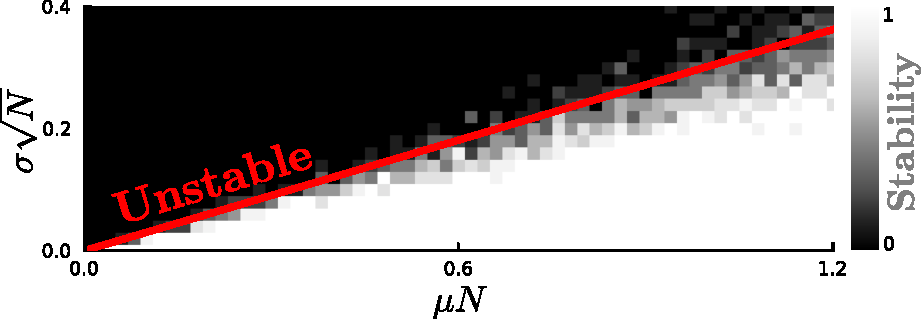
\includegraphics[width=.45\textwidth]{figs/beta1_5-S50-N10-diversity.pdf}
    \caption{For a system in the ``anti-May" phase, an increase in $N$,
    corresponding to moving along $\sqrt{N}$ in the $(\sigma \sqrt{N},\mu N)$ plane, will be stabilizing rather than destabilizing.
    Here we show results from the numerical resolution of the dynamical system \eqref{dynamics}. Stability is defined as full stable coexistence. The red line is computed obtained using DMFT and the generalized stability condition $N\langle (\sigma/\psi)^2\rangle < 1$.
    Parameters values are $\alpha=1$, $\beta=1.5$,
    $\gamma=1$, $N=50$ and $10$ replicates for the simulations.}
    \label{fig: stability line + sims}
\end{figure}

Stability of the equilibrium requires that $\mathcal{D}$ be entirely contained in the left half-plane (all eigenvalues have negative real part). For this, it is no longer sufficient that $\psi(x_i^*) > 0$ for each $i$: we must also have that $0\notin \mathcal{D}$, hence from \eqref{eq: domain}:
\begin{equation}
    \sum_{i=1}^N \Big(\frac{\sigma}{\psi(x_i^*)}\Big)^{2}
    < 1.
    \label{eq: random-stability}
\end{equation}
In the GLV model, $\psi(x) = \mu-\mu_s$ (independently of $x$) and we recover the classical condition $\sigma\sqrt{N} < (\mu_s-\mu)$ \footnote{In fact, the same condition holds when $f$ and $g$ are power laws with the same exponent.}. With more general power laws, the dependence on equilibrium values $x_i^*$ does not cancel out, and one must gain information about the distribution of equilibrium values $P(x_i^*)$ to assess the stability condition \eqref{eq: random-stability}.